\documentclass[10pt]{article}
%\documentclass[review]{siamart0516}
%\usepackage[utf8]{inputenc}
\usepackage[T1]{fontenc}
\usepackage{lmodern}
\usepackage{subfig}
%\usepackage[latin1]{inputenc}
\usepackage[english]{babel}
\usepackage{fullpage}
\usepackage{multirow}
%\usepackage{amsmath,amssymb,psfrag, amsthm}
\usepackage{amsmath,amssymb,psfrag}
\usepackage{graphicx}
\usepackage{listings}
\usepackage{paralist}
\usepackage{appendix}
%\usepackage{natbib}
\usepackage{amsfonts}
\usepackage{subfig,color}
\usepackage{comment} 
\usepackage{enumerate}
\usepackage{cancel}
\usepackage{footnote}
%\makesavenoteenv{tabular}
%\usepackage{helvet}
%\usepackage{algorithm}
%\usepackage{algorithmicx}
%\usepackage{algpseudocode}
\usepackage{epstopdf}
\usepackage{tikz,tikz-cd}
\usepackage{listings}
\usepackage{pgfplots,pgfplotstable}
\usetikzlibrary{pgfplots.groupplots}
\usetikzlibrary{positioning}
\usetikzlibrary[shapes,arrows,trees]
\usetikzlibrary{matrix,decorations.pathmorphing}
%\newcommand{\refalg}[1]{Algorithm~\ref{#1}}
%\newcommand{\refsec}[1]{Section~\ref{#1}}
%\newcommand{\reffig}[1]{Figure~\ref{#1}}
%\newcommand{\refsubfig}[1]{Figure~\subref{#1}}
%\newcommand{\reftab}[1]{Table~\ref{#1}}
%\newcommand{\refeqn}[1]{(\ref{#1})}
%\newcommand{\reflst}[1]{Listing~(\ref{#1})}
\newcommand{\refalg}[1]{\cref{#1}}
\newcommand{\refsec}[1]{\cref{#1}}
\newcommand{\reffig}[1]{\cref{#1}}
\newcommand{\refsubfig}[1]{\cref{#1}}
\newcommand{\reftab}[1]{\cref{#1}}
\newcommand{\refeqn}[1]{\cref{#1}}
\newcommand{\reflst}[1]{\cref{#1}}
\renewcommand{\d}{\mathrm{d}}
\newcommand{\re}[1]{(\ref{#1})}
\newcommand{\D}{\mathrm{D}}
\newcommand{\bb}[1]{\boldsymbol{#1}}
\def\sgn{\mathop{\rm sgn}}
\newcommand{\remark}[1]{{\color{red} #1}}
% THEOREMS ETC
\newcommand{\vect}[1]{\mathbf{#1} }
\newcommand{\order}[1]{\mathcal{O}(h^{#1})}
\newcommand{\code}[1]{{\tt #1}}
\renewcommand{\familydefault}{\sfdefault}
% -----------------------------------------------------------
% -----------------------------------------------------------
\lstset{backgroundcolor=\color[rgb]{0.92,0.95,1}}
\lstset{rulecolor=\color[rgb]{0.92,0.95,1}}
\lstset{numbers=left}
\lstset{basicstyle=\ttfamily\footnotesize}
\lstset{numberstyle=\footnotesize}

\def\dfdd#1#2{\frac{\partial#1}{\partial#2}}
\newcommand{\erf}{\, \mathrm{erf}}
\newcommand{\erfc}{\, \mathrm{erfc}}
%\renewcommand{\labelenumi}{[\arabic{enumi}]}

\newcommand{\dt}{\Delta t}
\newcommand{\dd}{\:\textrm{d}}
\newcommand{\CostFcn}{J}
\newcommand{\CostIntegrand}{g}
\newcommand{\param}{p}
\newcommand{\PDEConstr}{P}
\newcommand{\ModelN}{{\mathcal{F}}}
\newcommand{\ModelTLM}{F}
\newcommand{\Lagrangian}{{\mathcal{L}}}

%\normalsize
\pgfplotsset{compat=1.13}
\begin{document}
%\def\thefigure{\arabic{figure}}
%\def\thetable{\arabic{table}}

% TITLE AND AUTHOR --------------------------------
\title{PDE constrained optimization, error estimation and control with spectral elements using PETSc and TAO}
\vspace{1cm}
\author{Oana Marin, Emil Constantinescu, Barry Smith}
\date{\today}
\maketitle

Fitting observations to determine parameters, of either numerical or experimental nature, accelerating simulations throughout their long transients, identifiying  boundary conditions that satisfy certain observations, and many more such applications fall within the field of PDE constrained optimization and inverse problems. Despite their widespread aplicability inverse problems have been plagued by bottlenecks such as: ill-posedness, sensitivity to errors, high computational costs and these problems are also data intensive, placing high demands on the I/O and disk space. The current work aims to address these issues by leveraging the extensive range of methods available in both PETSc and TAO, to provide a framework for tackling large scale inverse problems in a robust fashion.

%The traditional approach to PDE constrained optimization is mathematically similar to the inverse problems approach however differs in terms of computational 

A PDE constrained optimization problem can be stated in two different ways according to the problem at hand: either by fully discretizing the entire KKT (Karush-Kuhn-Tucker) system, as is customary in the optimization community \cite{Haber_2007}, or by decoupling the direct problem and its adjoint and solving the optimization problem via a forward/backward timestepping loop, with appropriate initial and boundary conditions depending on the objective function.

We aim to address three of the five main strategies outlined in \cite{Brown_2008}. Specifically the core strategy in \cite{Brown_2008} is to proceed to the solution of inverse problem in a purely non-linear manner (a lot of work has previously relied on linearizations), and here we showcase a quasi-linear time dependent convection problem solved in PETSc with TAO. A second outlined challenge is to identify connections between uncertainty in the model and its underlying mathematical structure. This point can be interpreted in several ways and encompasses a series of problems, however we shall address this by means of error analysis of the numerical implementation and its impact on optimization. The last aspect we begin to grapple with is the gap between mathematical research and domain specific expertise, with a direct focus on computational fluid dynamics applications. Since the implementation is performed in the PETSc framework, a byproduct of this work is to open the road to a fourth strategy stated in \cite{Brown_2008}, which refers to the development of large-scale linear algebraic techniques that reliably capture the structure of ill-posedness. 

Given that inverse problems based on the full nonlinear underlying PDE as opposed to linearizations has been an issue for a long time, the data and computational intensity aspect has often been overlooked, however we addressed this in previous work \cite{schanen_2016}. The data intensity for nonlinear problems stems mainly from the nature of the backward in time component which depends at every time instance on its forward counterpart. A robust treatment for balancing the compute time versus trajectory storage has been already implemented in PETSc for certain time stepping routines for ordinary differential equations and in the current work we explore/extend it further to PDEs. 

A known aspect in the PDE optimization community is that continuous derivations of the adjoint equation differ in nature from their discrete couterpart, and may subsequently provide a different gradient which affects the convergence of the optimization step. To surpass this issue we implemented a spectral element method in PETSc, which is the spatial discretization with the highest accuracy per grid point of all presently available numerical schemes. Another novelty factor this work intends to bring about is to equip the solvers with a combined space/time error analysis to facilitate studies on the impact of errors on the optimization step. The relevance of this addition cannot be stressed enough, since the errors in the gradient computation tend to slow the convergence rate of the optimization.

The material is organized as follows: the time dependent inverse problem is stated in a spatially unaware fashion, which allows for any operators such as diffusion, convection etc. As a prerequisite the main aspects of a spectral element method are presented together with a discussion on best implementation choices. A set of canonical test problems is explored in depth by describing the continuous adjoint versus the discrete adjoint, followed by an error analysis discussion. Results of the PETSc/TAO implementation are presented, together with an outlook on future work.


  
\section{Inverse problem\label{sec:inverse}}
The aim of this work is to estimate and control the error in the solution of PDE constrained optimization problems. %We consider Burger's equation \cite{ou_2011}
We will denote a generic PDE model by
\begin{eqnarray}
 u_t &=& \mathcal P[ u ] , \  x \in \Omega \\ \nonumber
   B[u|_{\partial \Omega}(t)]&=& u_b(t), \\ \nonumber
   u( x,0)&=& u_0( x),\nonumber
\label{eq:generic}\end{eqnarray} 
where $\mathcal P[ u ]$ is a stand-in operator for derivatives
controlling the spatial behaviour of the solution $u$. The boundary
condition $u_b$ is also provided with an operator $B[u]$ which can be
the identity for Dirichlet boundary conditions or a derivative for
Neumann, while $u_b(t)$ denotes whether the boundaries are
homogeneously or inhomogeneously satisfied, or whether they are time
dependent. This notation does not exclude periodic boundary
conditions. For simplicity of presentation we assume only homogeneous Dirichlet and/or periodic boundary conditions; i.e.  $u|_{\partial \Omega}(t)= 0.$

%Let us assume that we seek to find the initial condition $u_0$ such
%that we minimize a function
%
%\begin{align}
%  \label{eq:Cost:general}
%\CostFcn(u_0) = \int_0^T \CostIntegrand(u(t)) \dd t\,.
%\end{align}
%

In this work we will consider simple data assimilation problems  for which we seek the initial condition $u_0$ that leads at time $T$ to a solution
$u$ which matches a reference solution $u_d$. In practice $ u_d$  is not known over the entire domain $\Omega$, but in a subset region $\Omega_s\subset \Omega$ where sensors have been placed. However, for simplicity we construct a continuous function
$u_d$ to avoid regularization issues, and consider the sensor values $u_s$ to be a restriction of the destination vector $u_d$, i.e. $u_s=u_d|_{\Omega_s}$. 
A cost functional which minimizes the difference between $| u- u_d|$ while preserving convexity is
\begin{equation}
  J[u_0]=\int_{\Omega}(u- u_d)^2 \ \d \Omega \,.  \label{eq:Cost_general}
\end{equation}

The optimization problem we seek to solve is
\begin{eqnarray}
\min_{u_0} &&J[u_0], \quad s.t. \\ \nonumber
u_t&=&\mathcal{P}[u], \quad \text{with}\ u|_{t=0}=u_0\ , \text{and} \  B[u|_{\partial \Omega}(t)]= u_b(t)\ ,
\label{optimizationproblem}
\end{eqnarray}
where the partial differential equation is given by $\mathcal P$ and can be either advection-difussion, pure diffusion or other combinations.

\section{Prerequisites}
%Consider a time dependent partial differential equation with constant coefficients, given by the spatial operator $ \mathcal P(\mathbf u)$ and initial conditions $\mathbf g(\cdot)$ as
%\begin{eqnarray}
% \frac{\partial\mathbf u}{\partial t} &=&  \mathcal P(\mathbf u) \ , \mathbf x \in \Omega \\ \nonumber
%  \mathbf u|_{\partial \Omega}&=&0, \\ 
%  \mathbf u(0,t)&=&\mathbf g(\mathbf x) \ . \nonumber \label{eq:generic}
%\end{eqnarray} 

To transition from the strong form of the equation to the weak form we define the spaces
$$
L^2(\Omega)=\lbrace u :\Omega\rightarrow \mathbb R |\quad \bigg(\int_{\Omega} |u|^2 \d \Omega \bigg)^{1/2}<\infty\ \rbrace
$$
with the subspace
$$
H^1(\Omega)=\lbrace u \in L^2(\Omega) |\quad \frac{\partial u}{\partial \vect x} \ \text{in}\  L^2(\Omega)\ \rbrace
$$
and its subspace
$$
H^1_0(\Omega)=\lbrace u \in H^1(\Omega) |\quad \ u|_{\partial\Omega}=0 \ \rbrace
$$

We define the space
\begin{eqnarray*}
K  =   K (\Omega) & = & \lbrace \bigg(\int_0^T \int_{\Omega} |u|^2 \d \Omega \d t \bigg) < \infty | \\
                  &   &  \bigg(\int_0^T \int_{\Omega} |u_t|^2 \d \Omega \d t \bigg) < \infty | \\
                  &   &  \bigg(\int_0^T \int_{\Omega} |\frac{\partial u}{\partial \vect x}|^2 \d \Omega \dt \bigg) < \infty | \quad  u|_{\partial\Omega}=0 \rbrace.
\end{eqnarray*}
Unless otherwise indicated we will assume all functions in this manuscript are in $K$.
For the weak form of a partial differential equation we seek $ u $ in $K$ with the property that the residual is orthogonal to the set of all test functions,
that is
\[
\int_0^T \int_{\Omega} (\mathbf u_t-\mathcal P(\vect u)) \mathbf v \d \Omega \d t = 0
\]
for all $\mathbf v$ in $K$.

Example: Let $\mathcal P(\mathbf u) = \nu \Delta \mathbf u + \mathbf a  \nabla \mathbf u$, where $\nu$ is a parameter which represents the viscosity, and $\mathbf a$ is the advection velocity. Apply integration by parts to remove any second derivatives from the equation to obtain
\begin{equation}
\int_0^T \bigg( \int_{\Omega}\frac{\partial\mathbf u}{\partial t} \mathbf v \ \d \Omega + \int_{\Omega} \nu\nabla \mathbf u\ \nabla \mathbf v\ \d \Omega - \int_{\Omega} \mathbf a \cdot \mathbf v\ \nabla \mathbf u\ \d \Omega-
 \int_{\partial \Omega} \nabla \mathbf u \ \mathbf v\  \d \partial \Omega \bigg) \d t =0\label{eq:weakcd}
\end{equation}
The boundary term vanishes since $\mathbf u, \mathbf v \in K.$

In calculus the quantity of interest in determining extremum values of functions is the gradient. In functional analysis (calculus of variations) the functional
derivative plays a similar role in determining functions that provide the extremum of functionals. The functional derivative of
\[
F(p) = \int f(r,p(r),\nabla p(r)) \d r
\]
is defined to be the function (denoted by $ \frac{\partial F}{\partial p(r)}$) that satisfies
\[
\int \frac{\partial F}{\partial p(r)} \phi(r) \d r = \frac{\d}{\d \epsilon} \int f(r,p(r) + \epsilon \phi(r),\nabla p(r) + \epsilon \nabla \phi(r) ) \d r
\]
for all $ \phi(r)$ in some appropriate space. By the calculus of variations, a neccessary condition for a function to provide the local
minimum or maximum of a functional is that the functional derivative is zero.




\subsection{The Spectral Element Method}
\label{sec:sem}

Based on the weak form given by Equation~\ref{eq:weakcd} several discretizations are suitable, the finite element method, spectral element, continuous or discontinuous Galerkin, etc.
The spectral element method is a subclass of Galerkin methods, or weighted residual methods. 
The idea is to minimize the error of the numerical computation in the energy norm over a chosen space of polynomials. 

In the following we illustrate the spectral element discretization for the convection-diffusion equation Equation~\ref{eq:weakcd}, restricting ourselves to the one dimensional case
\begin{equation}
u_t - \nu\Delta u\ +a \nabla u=0\ . \label{eq:1dcd}
\end{equation}

In the case of a spectral element method the domain $\Omega=\cup_{e=1,M} \Omega_e $, is decomposed in $M$ nonoverlapping 
subdomains $\Omega_e$, termed elements, over which the data will be represented by orthogonal polynomials.

Let us now define $X=H^1_0(\Omega)^d$. The space of polynomials of order $N$ defined over an element $\Omega^e, \ e=1,\ldots, E$ is
$$
\mathbb P_{N,E}=\lbrace  \phi| \phi \in L^2(\Omega); \quad \phi|_{\Omega^e} \text{polynomial of degree} \leq N\rbrace
$$
Subsequently $X_N=X\cap  P_{N,E}^d$, where $d$ is the dimension of the problem.

In the polynomial space $X_N$ we expand the numerical solution $u(x)=\sum_i^N u_i(x)\phi_i$.
With this choice the solution as well as the test space function $v$ can be expressed as
\begin{equation}
u(\vect x)=\sum_{i=1}^N u_{i}\phi_i(\vect x)\ .
\label{eq:ansatz}
\end{equation}

The discrete point distribution $\mathbf x$ can be either a Chebyshev grid, or a Legendre grid, in either case the polynomials are orthogonal $(\phi_i, \phi_j)=\delta_{ij}$. 
For the moment we consider solely one dimensional problems and to proceed with the numerical discretization we plug Equation~\ref{eq:ansatz} into Equation~\ref{eq:weakcd} to obtain
\begin{equation}
\frac{\partial}{\partial t}\int \sum_{i=1}^N u_{i}\phi_i(x) \sum_{j=1}^N v_{j}\phi_j(x) \d \Omega_e + \int\sum_{i=1}^N u_{i}\phi'_i(x) \sum_{j=1}^N v_{j}\phi'_j(x) \d \Omega_e  +\int\sum_{i=1}^N u_{i}\phi_i(x) \sum_{j=1}^N v_{j}\phi'_j(x) \d \Omega_e =0 \ .
\end{equation}

With proper reordering this yields

\begin{equation}
\frac{\partial}{\partial t}\sum_{i,j=1}^N u_{i}v_{j}\underbrace{\int \phi_i(x)\phi_j(x) \d \Omega_e}_{M_{ij}} + \sum_{i,j=1}^N u_{i} v_{j}\underbrace{\int\phi'_i(x) \phi'_j(x) \d \Omega_e}_{K_{ij}} +\sum_{i,j=1}^N u_{i} v_{j}\underbrace{\int\phi'_i(x) \phi_j(x) \d \Omega_e}_{D_{ij}}  =0
\end{equation}

where $M_{ij}$ is the mass matrix and $K_{ij}$ is the stiffness matrix. If the same polynomial order expansion as in the Equation~\ref{eq:ansatz} is used for the mass matrix then due to the orthogonality properties of the polynomials the mass matrix is diagonal. A higher order polynomial expansion yields a full matrix, which may alleviate disperssive errors as mentioned in \cite{ainsworth2014}, however in the current work we do not consider such matters.

In algebraic form we can rewrite
\begin{equation}
\frac{\partial}{\partial t}\underline{v}^TM\underline{u} + \underline{v}^TK\underline{u}+\underline{v}^TD\underline{u}=0
\end{equation}

with $\underline{u}=(u_0,\ u_1, \ldots, u_N)$ and similarly $\underline v$ is the array of point values of the test function. 
Note that one can factor out $\underline v$ to obtain an ODE

\begin{equation}
M\frac{d \underline{u}}{d t} =- K \underline{u}+ D \underline{u} \label{eq:discrete}
\end{equation}

Presume  $\Omega_e = [a, \ b]$ and define the reference element $\hat{\Omega} = [-1, \ 1]$.
For $x\in \Omega_e$ and $r \in \hat{\Omega}$ the mapping from each element to the reference element is
$$x= a+ \frac{b-a}{r+1}\ .$$

This mapping introduces a scaling factor for each element as given by the Jacobian of the coordinate transformation.

%\subsubsection{Spectral operators and their implementation}



%And the change of variables reads
%$$\frac{dx}{dr
\begin{comment}
\section{ODE solutions}
\subsection{Convergence tests}
\subsection{Various Boundary conditions}

\subsection{Convection-Diffusion}
Consider the energy equation in non-dimensional form Equation~\ref{eq:energy_nondim}, this is a convection diffusion equation with the Laplacian term weighted by the P\' eclet number. For the simplicity of the presentation we make two changes 
\begin{itemize}
\item replace the advection velocity $\vect u$ by a constant velocity field $c$ that is divergence free
\item denote the temperature $T$ in the energy equation by $u$
\end{itemize}
The variational formulation of the Convection-Diffusion equation reads
\begin{eqnarray}\label{eq:Conv_diff}
\int_{\Omega}\frac{\partial u}{\partial t} \cdot v\d \Omega+ \int_{\Omega}(c \cdot \nabla u)\cdot  v\d \Omega\ &=& \frac{1}{Pe}\int_{\Omega} (\nabla\cdot \nabla  u)\cdot  v\d \Omega + \int_{\Omega}f\cdot v\d \Omega.
\end{eqnarray}
with $ u,\ v \ \in \  H^1_0(\Omega)$.

The terms in the convection diffusion equation can be further expanded to give
\begin{eqnarray}\label{eq:var_cd}
\int_{\Omega}\frac{\partial u}{\partial t} \cdot \vect v\d \Omega &=&\frac{\partial}{\partial t} \int_{\Omega}u \cdot \vect v\d \Omega\\
\int_{\Omega} \nabla\cdot \nabla u\cdot v\d \Omega &=&\int_{\Omega}  \nabla u\cdot \nabla v\d \Omega +\int_{\partial\Omega} v \nabla u \cdot \vect n\d\Omega
\end{eqnarray}


Let us now define $X=H^1_0(\Omega)^d$. The space of polynomials of order $N$ defined over an element $\Omega^e, \ e=1,\ldots, E$ is
$$
\mathbb P_{N,E}=\lbrace  \phi| \phi \in L^2(\Omega); \quad \phi|_{\Omega^e} \text{polynomial of degree} \leq N\rbrace
$$
Subsequently $X_N=X\cap  P_{N,E}^d$, where $d$ is the dimension of the problem.

In the polynomial space $X_N$ we expand the numerical solution $u=\sum_i^N u_i\phi_i$.
With this choice the solution as well as the test space function $\vect v$ can be expanded as
$$
u(\vect x)=\sum_{i=1}^N u_{i}\phi_i(\vect x)
$$

Given the choice of the polynomial space $X_N$ the boundary integral term in \ref{eq:var_cd} vanishes. Upon insertion of the ansatz into the variational formulation we have
\begin{eqnarray}\label{eq:cd_ansatz}
\int_{\Omega}\frac{\partial u}{\partial t} \cdot \vect v\d \Omega &=&\frac{\partial}{\partial t} \sum_i^N\sum_j^N v_i\bigg(\int_{\Omega}  \phi_i(\vect x) \cdot \phi_j(\vect x)\d \Omega u_j\bigg) \\
\int_{\Omega}(c \cdot \nabla u)\cdot  v\d \Omega\ &=&\sum_i^N\sum_j^N v_i\bigg (\int_{\Omega}(c \cdot \phi_i(\vect x)\cdot \nabla\phi_j(\vect x)  \d \Omega\bigg) u_j\ \\
\int_{\Omega} (\nabla\cdot \nabla  u)\cdot  v\d \Omega &=&\sum_{i=1}^N \sum_{j=1}^N v_{i}(\int_{\Omega}\nabla\phi_i(\vect x) \cdot \nabla \phi_j(\vect x)\d \Omega)u_j \\
\end{eqnarray}

To discretize the integrals in \ref{eq:cd_ansatz} we need to introduce a quadrature rule. For spectral accuracy the choice is the Gauss-Legendre quadrature
$\int_{-1}^1\phi(\vect x)\d x=\sum_k \rho_k\phi(x_k)$
where the quadrature points $x_k$ are given by the Gauss-Legendre-Lobatto points, and the weights $\rho_k$ are based on the Legendre polynomials as in \ref{dfm02}.
To start with we consider the one dimensional case and proceed to higher dimensions and curvilinear elements.

\subsubsection{One Dimensional case}
Let us first regard a one dimensional case on the domain $\Omega=[a\ b]$ and analyze one by one the terms in Equation~\ref{eq:cd_ansatz}. Since the quadrature rule is defined on the interval $[-1, \ 1]$ we map $x \in \Omega$ to $r\in [-1,\ 1]$ via $x=a+(b-a)(r+1)/2$ and take $L=b-a$.
The mass matrix is given by 
\begin{equation}
M_{ij}=\int_{\Omega}\phi_i(x) \phi_j(x)\d \Omega=\frac{L}{2}\int_{-1}^1\phi_i(r) \phi_j(r)\d r=\frac{L}{2}\sum_k \rho_k\phi_i(r_k) \phi_j(r_k)
\end{equation}
since $\phi_i(x_k) \phi_j(x_k)=\delta_{ij}$, $M$ is a diagonal matrix which holds on the diagonal the weights of the quadrature rule. In practice $M$ can also be used as an integration operator, therefore one can write $\int_{-1}^1f(x)\d x\approx Mf$

The stiffness matrix corresponding to the second order term is 
\begin{equation}
A_{ij}=\int_{\Omega}\phi'_i(\vect x) \phi'_j(\vect x)\d \Omega=\frac{L}{2}\int_{-1}^1\phi'_i(r) \phi'_j(r)\d r=\frac{L}{2}\sum_k \rho_k\phi'_i(r_k) \phi'_j(r_k)
\end{equation}
and the convection operator
\begin{equation}
C_{ij}=\int_{\Omega}c\phi_i(\vect x) \phi'_j(\vect x)\d \Omega=\frac{L}{2}\int_{-1}^1c(r)\phi_i(r) \phi'_j(r)\d r=\frac{L}{2}\sum_k c(r_k)\rho_k\phi_i(r_k) \phi'_j(r_k)
\end{equation}

This leads to the following spatial discretized system of equations
\begin{equation}\label{eq:advd}
M \frac{d u}{dt} = \, Au -Cu + M f, 
\end{equation}


\subsubsection{Two Dimensional case}
Consider $\Omega=[-1,\ 1]^2$ discretized in $N$ GLL points. Then the basis function $\pi_k(x_1,x_2)=\phi_i(x_1)\phi_j(x_2)$ where $i,j=1,\ldots,N$ and $k=i+(N+1)\cdot j$.

The ansatz on the solution 
$$u(x,y)=\sum_{i=0}^M\sum_{j=0}^N u_{ij}\phi_i(x)\phi_j(y)$$

To start with we introduce a notation for tensor product form of matrix multiplication
\begin{equation}
w_{ij}=\sum_{l=1}^M\sum_{k=1}^N a_{jl}b_{ik}u_{kl}
\end{equation}
In the tensor product notation $c_{ij}=\sum_{l=1}^M\sum_{k=1}^N a_{jl}b_{ik}$ can be written as $C=A\otimes B)$. By unrolling the vector $w_{ij}$ as $\underline{w}_{\hat{i}}$ with components given by the ordering $\hat{i}=i+M\cdot(j-1)$ and similarly for $u_{kl}$ we can expand the tensor matrix product as \footnote{this doesn't match the one before.. careful with N+1, N}

$$\underline{w}=(A\otimes I)(I\otimes B)\underline{u}$$

From this notation simpler cases arise such as
\begin{equation}
w_{ij}=\sum_{k=1}^N a_{ik}u_{kj}\quad \rightarrow \quad \underline{w}=
\end{equation}
\section{Data Structure for SEM in Petsc}
\label{sec:sem}


%\begin{equation}
%  \mathbf u(\mathbf x)|_{\Omega_e} = \sum_{i,j,k} u^e_{ijk}
%  \phi_i(x_1)\phi_j(x_2)\phi_k(x_3)\ ,
%\end{equation} 

\label{sec:Spectral and Pseudo-spectral}
\end{comment}



\section{PDE constrained optimization}

Two main approaches are available when dealing with PDE-constrained optimization problems; both can be cast in a Lagrange-multipliers framework. Although the Lagrange-multipliers framework is not the sole path to solution for these types of optimization problems we choose it here for consistency, furthermore it offers a suitable way to illustrate the connections between continuous and discrete adjoints.

Variational calculus allows us to obtain a direct derivation of the adjoint equations, which are weakly decoupled from the forward PDE. By weakly decoupled in this context we mean that the backward and forward problems can be regarded as two independent PDEs where the backward problem is tied to the forward via initial conditions, boundary conditions as well as the advection velocity in the case of nonlinear problems.

In the examples we consider here an objective function that is  restricted to the final time horizon which implies that in Equation\ref{eq:Cost_general} we have $\mathcal{J}[u_0]=\int_{\Omega}( u[T]- u_d)^2 \ \d \Omega$. 

We sum up in Table~\ref{sum} the approaches available for PDE constrained optimization, outlining the current work and subsequently proceeding to the necessary derivations.

\begin{table}
\centering
\begin{tabular}{|r|c|c|}
  \hline
   & KKT system & Adjoint looping \\
  \hline\hline
  Discrete Adjoint & TAO\footnotemark
   & Current work (PETSc) \\ 
  Continous Adjoint& to be developed & Current work (MATLAB)\\
  \hline
\end{tabular}
\caption{PDE constrained optimization strategies.}\label{sum}
\end{table}
\footnotetext{\texttt{/petsc/src/tao/pde\_constrained/}}
\subsection{Variational calculus using the continous adjoint\label{sec:adj:continuous}} 

To derive the gradient used in the backward step we set up the Lagrangian, where $v$ plays the role of the Lagrangian multiplier
$$\mathcal{L}[ u,  v]=\int_{\Omega}( u[T]- u_d)^2 \ \d \Omega +\int_0^T\int_{\Omega} P[ u]  v \ \d \Omega \d t $$

\begin{comment}
+ \int_0^T\int_{\Gamma}  v_b  ( u-  u_b) \ \d \Gamma \d t
%
\footnote{Chain rule for $f=g\circ h$, g must be Frechet and if h' is Frechet or Gateaux so is f.}
%
\footnote{Riesz theorem: Let T be a functional on H then the Frechet derivative $T'(x)$ is given by
$T'(x) v= (\nabla T, v)$ for $\forall v \in H$.}
%
\end{comment}

Focusing on the term $\mathcal P[u]$ and presuming it stands for a diffusion operator we rewrite
\begin{eqnarray}
\int_0^T\int_{\Omega} P[u]  v \ \d \Omega \d t &=&
\int_0^T\int_{\Omega} \frac{d u}{d t}  v \ \d \Omega \d t+ \int_0^T\int_{\Omega} \nu\Delta  u \cdot  v \ \d \Omega \d t+\int_0^T\int_{\Omega}  f( x)   v \ \d \Omega \d t \\ \nonumber
&=& \int_{\Omega} u v \ \d \Omega|_0^T -
\int_0^T\int_{\Omega}
 \frac{d v}{d t}  u \ \d \Omega \d t+ \int_0^T\int_{\Gamma}(\nabla  u\cdot  v-  u\cdot \nabla v) n\ \d \Gamma \d t + \\ \nonumber
 && \int_0^T\int_{\Omega} \nu\Delta  v\cdot   u \ \d \Omega \d t \\ \nonumber
 &=& 
\int_0^T\int_{\Omega}
(- \frac{d v}{d t}  +\nu\Delta  v)\cdot   u\ \d \Omega \d t+\int_{\Omega} u v |_0^T \ \d \Omega
+ \int_0^T\int_{\Gamma}(\nabla  u\cdot  v-  u\cdot \nabla v) n\ \d \Gamma \d t \\ \nonumber
\end{eqnarray}
here $\Gamma=\partial \Omega$ is the boundary of the domain.

Grouping now the time dependent terms we have
\begin{eqnarray}
\mathcal{L}[ u, u_0,v]&=&\int_{\Omega}( u[T]- u_d)^2 + \int_{\Omega} u[T] v[T] - u[0] v[0]\ \d \Omega+\int_0^T\int_{\Omega} \overline{P}[ v]  u \ \d \Omega \d t + \\ \nonumber
 && \int_0^T\int_{\Gamma}(\nabla  u\cdot  v-  u\cdot \nabla v) n\ \d \Gamma \d t
\end{eqnarray}

Here we denote by $\overline{\mathcal P}$ the reverse mode which is reversed in time, i.e. $\overline{\mathcal P}[u(x,t)]=-\overline{\mathcal P}[u(x,-t)]$ and determines the backward heat equation in this case. 

In order to take a derivative of a functional we need to make use of the Riesz representation theorem, which states that for a functional $\mathcal J$, the derivative is $d \mathcal J[u]/dv=(u,v)(=\int_{\Omega} u\cdot v \ d \Omega)$. Considering now each partial derivative individually we have for the Lagrangian
\begin{eqnarray}
\nabla_u \mathcal L&=&- \frac{\partial v}{\partial t}  +\nu\Delta  v \\ \nonumber
\nabla_{u_0} \mathcal L&=&- v[0]\\ \nonumber
\nabla_{u_T} \mathcal L&=&2( u[T]- u_d)+ v[T]\\ \nonumber
\label{eq:bcs_ics}
\end{eqnarray}

The last two partial derivatives are responsible for initial conditions for the forward and for the reverse (adjoint) problem.

\subsection{Discrete Adjoint \label{sec:adj:discrete}} 

In a discrete setting now the solution space becomes from $L^2(\Omega;[0,T])$ the discrete $\mathbb{R}^{n(N+1)}$, where we have $n$ components and $N$ time
steps. The inner product in this space is defined as $\langle u , v
\rangle = \sum_{k=0}^N \sum_{i=1}^{n} u_k^{(i)} v_k^{(i)} =
\sum_{k=0}^N  (u_k)^T v_k$; i.e., $k$ indexes all times and $i$ all
spatial locations. Then the adjoint of $A$ is $A^*$ s.t. $\langle A u , v
\rangle = \langle u , A^* v \rangle $, $u,v \in \mathbb{R}^{n(N+1)}$.

Let us assume we have a time-dependent problem such as Equation~\ref{eq:1dcd} where again we omit the convective term, since it far less problematic. In semi-discrete form we write
%
\begin{align}
  \label{eq:semi:discrete:form}
\frac{\partial u}{\partial t} = f(u,p,t)\,, 
\end{align}
which is identical with Equation~\ref{eq:generic}, with the difference that now we need an explicit definition of the spatial operator at every time step so we took $f(u,p,t)=\mathcal P[u,p](t)$, previously it was sufficient to consider the dependency of $\mathcal P$ on $u$. Note that in fact the optimization parameter remains $\param=u_0$, however we shall write $p$ to avoid confusion with the discrete timestep $u_0$. 
The discrete process now reads
%
\begin{align}
   \label{eq:discrete:form}
u_{k+1} = \ModelN(u_{k};\param,\dt)\,,~ k=0,1,\dots, N\,.
\end{align}
%
Furthermore, consider a discretization of the cost function
Equation~\ref{eq:Cost_general} where for brevity we set the notation $g(u)=\int_{\Omega} (u-u_d)^2 \d \Omega$. We set for instance a simple Riemann summation
$\CostFcn(u_0) = \dt\sum_{k=2}^{N-1}  g(u_k)$. The optimization problem is therefore
%
\begin{align}
  \label{eq:discrete:optim}
\min_{u_0,u_{k+1} - \ModelN(u_{k})=0\,,~ k=0,1,\dots, N} \CostFcn(u_0)\,.
\end{align}
%
The Lagrangian function for Equation~\ref{eq:discrete:optim} is
%
\begin{align}
  \nonumber
\Lagrangian[u,\lambda,p] = \CostFcn(u_0) - \sum_{k=0}^{N-1} \lambda_k^T
\left(u_{k+1} - \ModelN(u_{k})\right)\,. 
\end{align}
%
The gradient with respect to $\param$ is given by:
%
\begin{align}
  \nonumber
\nabla_\param\Lagrangian =\nabla_\param \CostFcn(u_0) - \sum_{k=0}^{N-1}
\lambda_k^T \left(\frac{\partial u_{k+1}}{\partial \param} - \ModelTLM
\frac{\partial u_{k}}{\partial \param}\right)\,,
\end{align}
%
where $\ModelTLM_k = \left. \frac{\partial \ModelN(u;\param)}{\partial
  u}\right|_{u=u_k}$ is the tangent linear model. It follows that
%
\begin{allowdisplaybreaks}
\begin{align}
  \nonumber
  \nabla_\param
  \Lagrangian =&\dt \sum_{k=1}^{N} \left.
  \frac{\partial
  \CostIntegrand(u)}{\partial u}\frac{\partial u}{\partial \param}
  \right|_{u=u_k}
- \sum_{k=0}^{N-1} \lambda_k^T \frac{\partial u_{k+1}}{\partial
  \param}  + \sum_{k=0}^{N-1}
\lambda_k^T \ModelTLM \frac{\partial u_{k}}{\partial \param}
\\
%%%
\nonumber
=& \dt\sum_{k=1}^{N}  
\frac{\partial
  \CostIntegrand(u_k)}{\partial u} \frac{\partial u_k}{\partial \param}-
\sum_{k=1}^{N} \lambda_{k-1}^T \frac{\partial u_{k}}{\partial \param}
+ \sum_{k=0}^{N-1} \lambda_k^T \ModelTLM \frac{\partial
  u_{k}}{\partial \param}
\\
%%%
\nonumber
=&\sum_{k=1}^{N-1}  \left(  \dt \frac{\partial
  \CostIntegrand(u)}{\partial u}  -  \lambda_{k-1}^T  +  \lambda_k^T
\ModelTLM \right) \frac{\partial u_{k}}{\partial \param} + \dt \frac{\partial
  \CostIntegrand(u_N)}{\partial u} \frac{\partial u_{N}}{\partial
  \param} -  \lambda_{N-1}^T \frac{\partial u_{N}}{\partial \param} +
\lambda_0^T \ModelTLM \frac{\partial   u_{0}}{\partial \param}
\\
%%%
\nonumber
=&\sum_{k=1}^{N-1}  \left(    - \lambda_{k-1}   +  \ModelTLM^T
\lambda_k +\left(\dt\frac{\partial
  \CostIntegrand(u)}{\partial u}\right)^T \right)^T \frac{\partial u_{k}}{\partial \param} + \dt \frac{\partial
  \CostIntegrand(u_N)}{\partial u} \frac{\partial u_{N}}{\partial
  \param} -  \lambda_{N-1}^T \frac{\partial u_{N}}{\partial \param} +
\lambda_0^T \ModelTLM \frac{\partial   u_{0}}{\partial \param}
\\
%%%
\nonumber
=&\sum_{k=1}^{N-1}  \left(  -   \lambda_{k-1}   +  \ModelTLM^T
\lambda_k + \left(\dt\frac{\partial
  \CostIntegrand(u)}{\partial u}\right)^T \right)^T \frac{\partial
  u_{k}}{\partial \param} + \left(\dt \frac{\partial 
  \CostIntegrand(u_N)}{\partial u}  -  \lambda_{N-1}^T\right)
\frac{\partial u_{N}}{\partial \param} +
\lambda_0^T \ModelTLM \frac{\partial u_{0}}{\partial \param}\,.
\end{align}
\end{allowdisplaybreaks}
%
Now choose $\lambda$ so that the so called adjoint system, $\lambda_{k-1}   -  \ModelTLM^T
\lambda_k + s_k$ is satisfied and the boundary conditions vanish so
that $\lambda_0 = \nabla_\param \CostFcn(u_0)$, where $s_k$ is the
source term.

\paragraph{Adjoint for forward Euler.} The numerical algorithm for
forward Euler satisfies:
%
\begin{align}
  \label{eq:FE}
  %\nonumber
  &u_{k+1}=u_k + \dt f(u_k)= \ModelN(u_k;\param,\dt)\,,\\
  \nonumber
  &\left. \ModelTLM \right|_{u=u_k} =\ModelTLM_k = (I + \dt
  J(t_k,u_k,\param))\,.
\end{align}
%
The discrete adjoint for this scheme is then
%
\begin{align}
\nonumber
&\lambda_{k-1}   -  \ModelTLM^T \lambda_k + s_k =0
\\
\nonumber
&\lambda_{k-1} = \left(I + \dt J(t_{k},u_{k},\param) \right)^T \lambda_k -
s_k
\\
\label{eq:FE:adjoint}
&\lambda_{k-1} =  \lambda_k + \dt J(t_k,u_k,\param)^T \lambda_k - s_k\,.
\end{align}
%
Equation \eqref{eq:FE:adjoint} describes the adjoint of the forward
Euler method; it goes backward in time (from step $N$ to $0$) and it
is initialized with $s_N$.


\paragraph{Adjoint for backward Euler.} The numerical algorithm for
backward Euler satisfies:
%
\begin{align}
  \label{eq:BE}
  %\nonumber
  &u_{k+1}=u_k + \dt f(u_{k+1})= \ModelN(u_k;\param,\dt)\,,\\
  \nonumber
  &\left. \ModelTLM \right|_{u=u_k} =\ModelTLM_k = \left(I - \dt
  J(t_{k+1},u_{k+1},\param)\right)^{-1}\,.
\end{align}
%
The discrete adjoint for this scheme is then
%
\begin{align}
\nonumber
&\lambda_{k-1}   -  \ModelTLM^T \lambda_k + s_k =0
\\
\nonumber
&\lambda_{k-1} = \left(I - \dt J(t_{k-1},u_{k-1},\param)^T \right)^{-1} \lambda_k -
s_k
\\
\nonumber
&\left(I - \dt J(t_{k-1},u_{k-1},\param)^T \right) \lambda_{k-1} = \lambda_k -
\left(I - \dt J(t_{k-1},u_{k-1},\param)^T \right) s_k\\
\label{eq:BE:adjoint}
& \lambda_{k-1} = \lambda_k + \dt J(t_{k-1},u_{k-1},\param)^T
\lambda_{k-1} -
\left(I - \dt J(t_{k-1},u_{k-1},\param)^T \right) s_k\,.
\end{align}
%
Equation \eqref{eq:BE:adjoint} describes the adjoint of the backward
Euler method; it goes backward in time (from step $N$ to $0$) and it
is initialized with $s_N$.

\subsection{Using Adjoints for Optimization}

We want a somewhat general problem, but not too general.

The optimization problem \ref{optimizationproblem} is posed as an optimization of a functional subject to a time dependent PDE constraint.
Conside the (more general than presented before)
optimization problem with the constraint posed in weak form
\begin{eqnarray}
  \min_{u \in K} \int_{\Omega}g(u(T)) \ \d \Omega + \int_0^T\int_{\Omega}G(u) \ \d \Omega \d t \quad s.t. \\ \nonumber
  \int_0^T \int_{\Omega} v^T( u_t- P( u))  \d \Omega \d t = 0, \quad \forall v \in K.
\label{newoptimizationproblem}
\end{eqnarray}


In this section we demonstrate how, using the functional analysis equivalent of Lagrange multiplies, it can be reformated and solved as
an unconstrained optimization. This approach is known as the adjoint state method. 
The unconstrained problem
\begin{eqnarray}
  \min_{u \in K, v \in K} \Lagrangian(u,v) = \min_{u \in K, v \in K} \int_{\Omega}g(u(T)) \ \d \Omega + \int_0^T\int_{\Omega}(G(u)  +   v^T ( u_t- P( u))) \d \Omega \d t
\label{unconstrainedoptimizationproblem}
\end{eqnarray}
has a stationary point for each extremum of the original problem (plus possibly additional stationary points). In this formulation the $ v$ play the role of
Lagrange multipliers. We integrate by parts and for clarity explicitly include $ u(0) $ and $ u(T) $ in the arguments of the Lagrangian resulting in
\[
\Lagrangian(u,v,u(0),u(T)) =  \int_0^T\int_{\Omega}(G(u) -  v^T_tu - \tilde{P}( v)  u) \d \Omega \d t + \int_{\Omega} (g(u(T)  + v(T)^Tu(T) - v(0)^Tu(0)) \d \Omega.
\]
The integration by parts is used to shift the $u$ outside of the $P()$ so that the result is linear in $u$; this is not possible to do for all forms of $p()$ but presumably in those cases one can
directly apply the definition of the functional derivative to the original form.
Now using the definition of the functional derivative we obtain
\[
\int_0^T\int_{\Omega} \frac{\partial \Lagrangian(u,v,u(0),u(T))}{\partial u}\phi = \int_0^T\int_{\Omega} (\frac{\partial G}{\partial u}(u) -  v_t - \tilde{P}(v))\phi \d \Omega
\]
\[
\int_{\Omega} \frac{\partial \Lagrangian(u,v,u(0),u(T))}{\partial u(0)}\phi = \int_{\Omega}  - v(0)\phi \d \Omega
\], and
\[
\int_{\Omega} \frac{\partial \Lagrangian(u,v,u(0),u(T))}{\partial u(T)}\phi = \int_{\Omega} (\frac{\partial g}{\partial u(T)}(u(T)) - v(T))\phi \d \Omega.
\] 
In strong form the resulting equations are
\begin{eqnarray}
\nabla_u \mathcal L&=&- \frac{\partial v}{\partial t}  +\nu\Delta  v = 0\\ \nonumber
\nabla_{u_0} \mathcal L&=&- v[0] = 0\\ \nonumber
\nabla_{u_T} \mathcal L&=&2( u[T]- u_d)+ v[T] = 0.\\ \nonumber
\label{eq:bcs_ics}
\end{eqnarray}


Example convection-diffusion method problem. 

\subsubsection{Semi-discrete Adjoints}

In this section we use $ \overline{u} $ to represent a vector of finite element coefficients (which are still time dependent) and we use
the {\em denominator layout} for derivatives, i.e. vectors are column oriented as are gradients, a byproduct of this notation is that
$ \frac{\partial \overline{v}^T A \overline{u}}{\partial \overline{u}} = A^T \overline{v}.$

Instead of first minimizing the Lagrangian via the functional derivative one
can first discretize in space and then optimizing. So rewrite \ref{unconstrainedoptimizationproblem}, after discretizing in space, resulting in

\begin{eqnarray}
  \min_{\overline{u} \in R^{n}, \overline{v} \in R^{n}} \Lagrangian(\overline{u},\overline{v},\overline{u}(0),\overline{u}(T) =  \min_{\overline{u} \in R^{n}, \overline{v} \in R^{n}} \int_0^T(\overline{G}(\overline{u})  -   \overline{v}_t^TM\overline{u}  - \overline{v}^T \overline{P}(\overline{u})) \d t + \overline{g}(\overline{u}(T)) \d  t + \overline{v}(T)^TM\overline{u}(T) - \overline{v}(0)^TM\overline{u}(0).
\end{eqnarray}
Now take the functional derivative only with respect to time resulting in
\[
  \int_0^T \frac{\partial \Lagrangian(\overline{u},\overline{v},\overline{u}(0),\overline{u}(T))}{\partial \overline{u}}\overline{\phi} = \int_0^T (\frac{\partial \overline{G}}{\partial \overline{u}} -  M \overline{v}_t  - \frac{\partial \overline{P}}{\partial \overline{u}}(\overline{u})^T\overline{v})\overline{\phi} \d  t.
  \]
  \[
  \frac{\partial \Lagrangian(\overline{u},\overline{v},\overline{u}(0),\overline{u}(T))}{\partial \overline{u(0)}} = -M \overline{v}(0)
  \]
  \[
  \frac{\partial \Lagrangian(\overline{u},\overline{v},\overline{u}(0),\overline{u}(T))}{\partial \overline{u(T)}} = \frac{\partial \overline{g}}{\partial \overline{u}(T)}(\overline{u}(T)) - M \overline{v}(T)) -M \overline{v}(T). 
  \]
  In strong form the equations can be written as

Example convection-diffusion method problem.  

\subsubsection{Discrete Adjoints}

Oana will rewrite Emil's discrete stuff using the notation for continous and semi-discrete approaches showing how similar it is.

Example convection-diffusion method problem.

\subsubsection{Discuss sparsity pattern of Euler Lagrangian equations and how the triangular format allows adjoints to work}

\subsubsection{Parallel in time methods, i.e. keep all the unknowns from all timesteps in one big ass problem}

\subsection{Nontrivial Boundary Conditions}

In the discussion above, for simplicity, we considered only periodic or homogeneous boundary conditions here we show how nontrivial boundary conditions can be handled. 

\section{PETSc implementation}

PETSc has data structures and algorithms for both time integration via TS and optimization, via TAO.
For spatial discretization the user needs to prove the matrices that arise from the space dependent operators ($\nabla,\ \Delta,\ \nabla \times$, etc) equipped with the aproppiate boundary conditions. The time step routines can integrate forward in time using the integrator of choice, multistage, multistep, and several other more exotic time integrators.

The gradient based optimization can be performed using adjoint information, or as a coupled KKT system \cite{Haber_2007}. Here we showcase the adjoint based approach, which as illustrated in Figure~\ref{fig:algorithm} consists of two solvers, one forward and one backward in time.

\begin{figure}
\begin{center}
 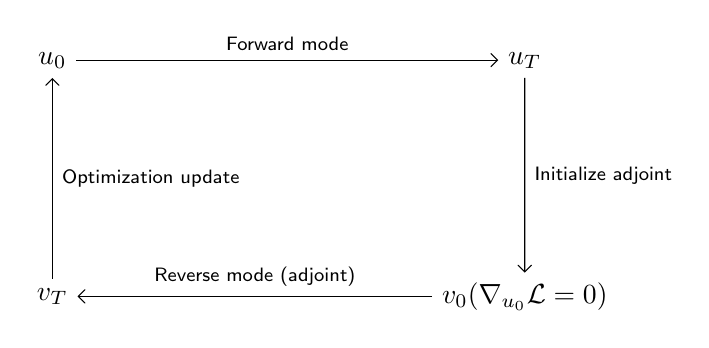
\begin{tikzpicture}[scale=3.0]
\node (A) at (0,1) {$u_0$};
\node (B) at (2,1) {$u_T$};
\node (C) at (2,0) {$v_0 (\nabla_{u_0} \mathcal L=0)$};
\node (D) at (0,0) {$v_T$};
\path[->,font=\scriptsize,>=angle 90]
(A) edge node[above]{Forward mode} (B)
(D) edge node[right]{Optimization update} (A)
(B) edge node[right]{Initialize adjoint} (C)
(C) edge node[above]{Reverse mode (adjoint)} (D);
\end{tikzpicture}
\end{center}
 \caption{Workflow for compression and restoring the solution.} 
  \label{fig:algorithm}
\end{figure}
\lstset{language=C,numbers=left,
    stepnumber=5,
    showstringspaces=false,
    tabsize=2,
    breaklines=true,
    breakatwhitespace=true}
\begin{lstlisting}[caption=PETSc code for PDE constrained optimization via adjoints, label=codemat]

  //TS object initialized previsouly
  ierr = TSSetSaveTrajectory(appctx->ts);CHKERRQ(ierr);
  ierr = TSSolve(appctx->ts,appctx->dat.curr_sol);CHKERRQ(ierr);
  
  // Compute the L2-norm of the objective function f
  ierr = VecDuplicate(appctx->dat.obj,&temp);CHKERRQ(ierr);
  ierr = VecCopy(appctx->dat.obj,temp);CHKERRQ(ierr);
  ierr = VecAXPY(temp,-1.0,appctx->dat.curr_sol);CHKERRQ(ierr);
  
   // Initial conditions for the adjoint integration, given by 2*obj'=temp    
  ierr = VecScale(temp, -2.0);
  ierr = VecCopy(temp,appctx->dat.grad);CHKERRQ(ierr);
  
  // Compute obective function
  ierr = VecPointwiseMult(temp,temp,temp);CHKERRQ(ierr);
  ierr = VecDot(temp,appctx->SEMop.mass,f);CHKERRQ(ierr);
  
  //Set gradient and objective function
  ierr = TSSetCostGradients(appctx->ts,1,&appctx>dat.grad,NULL);CHKERRQ(ierr);
       
  //Solve adjoint step
  ierr = TSAdjointSolve(appctx->ts);CHKERRQ(ierr);
  ierr = VecCopy(appctx->dat.grad,G);CHKERRQ(ierr);
  
  //get solution status from TAO
  ierr=  TaoGetSolutionStatus(tao, &its, &ff, &gnorm, &cnorm, &xdiff, &reason);
\end{lstlisting}
\begin{figure}[!ht]
\centering
\includegraphics[width=0.4\textwidth]{Cost_decay.eps}
%\label{fig:wingfull_est}}
\caption{Cost function decay.}
\label{fig:decay_cd}
\end{figure}

\begin{figure}[!h]
\centering
\subfloat[Initial condition(black) and desired profile(red)]
{\includegraphics[width=0.47\textwidth]{IC_OBJ.eps}
\label{fig:ic_obj}}
\quad
\subfloat[Result of Optimization problem for convection-diffusion for time horizon T=1, (blue) objective function, (red) optimal solution, (black) initial condition at first iteration]
{\includegraphics[width=0.47\textwidth]{optimization.eps}
\label{fig:opt_cd}}
\caption{Optimal initial conditions for a convection-diffusion problem.}
\end{figure}
\section{Results}

In the current framework we consider a set of problems in one dimension: diffusion, convection-diffusion, and diffusion with a discretely discontinous objective function. All spatial operators are discretized using the spectral element method, implemented now in PETSc, and the time integration is based on the TS capability of PETSc.

To be noted that diffussion domainated problem such as the ones studied here are highly ill-conditioned since small perturbations in the initial conditions smooth away quickly. This implies that multiple initial conditions lead to the same final solution, which proves to be a challenge when solving inverse problems.


\subsection{Advection-Diffusion}
We consider Equation~\ref{eq:1dcd} and seek $u_0$ which minimizes $\int (u[T]-u_d)^2\d \Omega$. 
The advection diffusion problem admits and analytical solution $u(x,t)=u_0(x-at)e^{-\nu t}$. The initial condition chosen here is a Gaussian convecting to the left side of the domain and the desired state we wish to optimize for is given by $u(x,T)$, we refer to $T$ as the time horizon of the problem. The paramters chosen here are advective velocity $a=0.05$ and viscosity $\nu=0.001$.

In Figure~\ref{fig:ic_obj} we illustrate both the initial condition and desired solution we seek to attain at time horizon $T$. The cost function decay versus the number of iterations required for finding the initial condition $u_0$ is illustrated in Figure~\ref{fig:decay_cd}. For an admissible error in the solution of $10^{-8}$ we obtain the final optimal in Figure\ref{fig:opt_cd}. The optimization algorithm used here is quasi-Newton algorithm, specifically Limited Memory Variable Metric (\texttt{LMVM}), and the timestepper is an explicit Runge-Kutta of 3rd order accuracy.


\subsection{Diffussion}

A diffusion problem with periodic boundary conditions and viscosity parameter $\nu=0.001$ is considered over the domain $[0,1]$. The domain is discretized in 5 elements each of polynomial order $N=8$ and the time horizon of the forward problem is $T=1$. We distinguish two cases one where the objective function is smooth, and the desired end state $u_d$ is discretized over the entire domain, and a second case where $u_d$ is not available at every grid in the domain, but a scattered selection of points.

We establish an analytical solution to the heat equation: 
\begin{equation}
u(x,t)=\sin(2\pi x)e^{-4\pi^2\mu t}+\cos(4\pi x)e^{-16\pi^2\mu t}
\label{eq:heatex}
\end{equation}

We choose the objective function to be a solution to the heat equation, i.e. in Equation~\ref{eq:heatex}, $u_d=u(x,T_a)$, where we set $T_a=3.0$. For the time horizon of the problem we choose $T=1.0$ and seek again to optimize for the initial condition, we minimize $\mathcal J[u_0]=\int_{\Omega} (u[T]-u_d)^2 \d \Omega$. The initial condition we start from is $u_0=u(x,0)=(\sin(2\pi x)+\cos(4\pi x))$. Since the time horizon is $T=1.0$ and the objective function is the solution at $T_a=3.0$ we can compare the result of the optimization with the exact solution at $u(x,T_a-T)$, and identify the behaviour of the errors.

\paragraph{Continous/Dense objective function} 
The smooth continous case is illustrated in Figure~\ref{fig:ic_obj_heat}, and Figure~\ref{fig:opt_heat}. We note a difference between the optimal and the objective, which is only natural given that the initial optimal condition has to decay for a time $T$ to reach $u_d$.

Comparing now the error of the optimal solution stemming from the optimization $u_0^{opt}$ and the analytical solution at the same time instance $u(x,T_a-T)$ we note in Figure~\ref{fig:opt_heat} that the error between the two is higher than the threshold imposed on the optimization. This can be easily explained by analyzing the errors incurred by the PDE solver which will always overtake the error in the optimization. Put simply if the PDE is resolved with an error $\epsilon$, then the optimization problem will be bound by the same error, $\vert u_0^{opt} -u(x,T_a-T)\vert \approx \epsilon $. 

In this case the PDE error is a compound of the space $\mathcal O(e{-\sigma N})$ error and time errors, which for a method of third order are $\mathcal O{dt^3}$. We performed a spatial error analysis on this problem, described in Section~\ref{sec:err}, and in Figure~\ref{fig:err_tot} we illustrate for this particular case the spatial error on a per element basis. The upper bound of the error the spatial error is given by the left most element in this discretization and is of magnitude $10^{-7}$. To observe this in the full optimization setup we chose a timestep of size $10^{-5}$, far lower than the stability requirements of the problem, and totally impractical for computational purposes, however revealing for the spatial error which we can see plateaus at $10^{-5}$, which we can consider to be within the round off vicinity of the spatial error. This is by no means an extensive study of errors, but a prerequiste to a fully fledged analysis of the interplay between the convergence of the optimization and the error of the underlying PDE.

\paragraph{Discrete/Sparse objective function}
The case where the objective is only a discrete set of points $N_s=\alpha\%N$, only a fraction $\alpha$ of the total spatial discretization $N$, is now considered. In this case the objective function becomes a fully discrete functional
$\mathcal J[u_0]=\sum_{i=1}^{N_s} (u^i[T]-u^i_d)^2 $ which needs to be regularized.

The regularization we consider here is 
$\Sigma[u_0]=\int_{\Omega} \nabla u \nabla u \d\Omega$, which leads to the modified objective function
$$\mathcal J_{reg}[u_0]= \mathcal J[u_0]+\Sigma[u_0] \ .$$

The intial condition of the reverse mode will now be, as in Equation~\ref{eq:bcs_ics}, given by $\nabla_{u_0} \mathcal J_{reg}[u_0] =\nabla_{u_0} \mathcal J[u_0]+\nabla_{u_0} \Sigma[u_0]=0 $.

For a choice $\alpha=80$, i.e. $N_s=0.8N$ uniformly distributed sensors, solving the optimization problem is similar to a least squares problems for the objective function, and we expect the fitting of the initial condition to have a higher deviation from the analytical solution. In Figure~\ref{eq:heatex} we note that the soltuion plateaus higher at a value of approximately $10^{-3}$, and several line searches at the first iteration are sufficent to acheive this result. The level at which this plateau is acheived is problem dependent and also can be impacted by the distribution of sensors as well as the number of sensors. Here for simplicity we chose the sensors to coincide with grid points, however in large scale applications they would be interpolated back and forth to the computational grid, which would additional errors to the problem.




\begin{figure}[!ht]
\centering
\subfloat[Result of Optimization problem for convection-diffusion for time horizon T=1, (blue) objective function, (red) optimal solution, (black) initial condition at first iteration]
{\includegraphics[width=0.47\textwidth]{Heatopt.eps}
\label{fig:ic_obj_heat}}
\quad
\subfloat[Cost function decay versus number of iterations]
{\includegraphics[width=0.47\textwidth]{Heat_decay.eps}
\label{fig:opt_heat}}
\caption{Optimal initial conditions for the heat equation with a smooth objective function, and time horizon T=1.}
\end{figure}



\begin{figure}[!ht]
\centering
\includegraphics[width=0.5\textwidth]{decayregvsc.eps}
\label{fig:opt_heatass}
\caption{Log-scale of error between analytical solution and optimal solution: (red) continous/dense objective functional, (blue) discrete/sparse objective functional. For the sparse objective we have a number of line searches performed in the first iteration, while the for the dense one only one line search per iteration was sufficient.}
\end{figure}

\section{Spatial error estimation}
\label{sec:err}
To assess the error incurred in the spatial discretization we use the a posteriori spectral error analysis suggested in \cite{Mavriplis1990}, and a lengthy review on the matter can be found in \cite{kopriva2009}. 

Considering the discrete solution $u_N\in X_N$ (the Hilbert space of polynomials of order $N$ defined in Section~\ref{sec:sem}), an extrapolated solution $\tilde u\in X_M$, a space of polynomials of order $M\gg N$ and the exact solution $u$ we can bound the error as
$$\Vert u - u_N\Vert \leq \underbrace{\Vert u-\tilde u\Vert}_{\text{extrapolation err.}} + \underbrace{\Vert \tilde u- \Pi_N \tilde u\Vert}_{\text{truncation err.}} + \underbrace{\Vert u_N-\Pi_N \tilde u\Vert}_{\text{quadrature err.}} \ ,$$
where $\Pi_h u$ is the projection of $u$ on a polynomial space of order $N$.

We can identify the terms in the error one by one as follows
\begin{itemize}
\item \textit{extrapolation error} -- the error incurred by extrapolating the solution to a higher order space (needed to identify the truncation error, this error is negligable)
\item \textit{truncation error} -- the error incurred by the truncation to a lower order space
\item \textit{quadrature error} -- the error of the quadrature used by discretizing the weak formulation.
\end{itemize}

The remaining two errors are withstanding and given that we are in a spectral element framework the projection on an orthogonal polynomial space exhibit spectral decay. A through derivation gives the leading order term of the truncation in the error bound to be $\epsilon_e$ with

$$\epsilon_e=\frac{a_N^2}{(2N+2)/2}\ , $$
where $a_N$ can be approximated from a least squares expansion to be $a_N=ce^{-\sigma N}$, $N$ is the number of degrees of freedom, $\sigma$ the slope of the decay and $c$ a scaling factor. 

The actual computational procedure is rather straightforward: we transform the signal into spectral space where the decay can be viewed as a linear function in log-scale and form there we compute both $\sigma$ and $c$.
This operation is performed per element and for a given signal such as the one in Figure~\ref{fig:err_tot} we obtain error bounds per element that are consistent with the signal fluctuations as illustrated in Figure~\ref{fig:err_tot}. As a general procedure we perform a least square fit in spectral space to identify the value of the parameter $\sigma$. To certify the consistency of the fit with the spectral decay we show in Figure~\ref{fig:err_spec} the estimated error decay versus the actual spectral error.




\begin{figure}[!ht]
\centering
\subfloat[Solution to the heat equation for a discretization of N=8 points over E=5 elements(red), and error bars in log scale (right y axis) per element computed via the error estimator(black).]
{\includegraphics[width=0.47\textwidth]{superpose.eps}
\label{fig:err_tot}}
\quad
\subfloat[Error computed per element. Sample elements 1:3 represented by different markers, spectral representation of the signal (red), error estimate (blue).]
{\includegraphics[width=0.47\textwidth]{specerr.eps}
\label{fig:err_spec}}
\caption{A posteriori error estimation for a spectral spatial discretization.}
\end{figure}



%
%\begin{figure}
%\begin{center}
% \begin{tikzpicture}[scale=2.0]
%\node (A) at (0,1) {$\mathbf u$};
%\node (B) at (1.5,1) {$T\mathbf u$};
%\node (C) at (1.5,0) {$T\tilde{\mathbf u}$};
%\node (D) at (0,0) {$\tilde{\mathbf u}$};
%\path[->,font=\scriptsize,>=angle 90]
%(A) edge node[above]{$DCT$} (B)
%(D) edge node[right]{$Error$} (A)
%(B) edge node[right]{$Truncate \rightarrow \texttt{Huffman\ encode}$} (C)
%(C) edge node[above]{$IDCT$} (D);
%\end{tikzpicture}
%\end{center}
% \caption{Workflow for compression and restoring the solution.} 
%  \label{fig:algorithm}
%\end{figure}
%
%\subsection{Algorithm}
%\begin{algorithm}
%\begin{algorithmic}[5]
%\Procedure{Setup}{}
%\State  {\tt T $\leftarrow$ DCT\_setup\_1d(p) }
%%\State {\tt M $\leftarrow$ build\_map($\text{mesh}_{\text{gll}})$}
%\EndProcedure
%\Procedure{Truncate}{}
%%\For {\tt k$\in$ $LocalEL_{id}(COMPnode)$} %\Comment{$ttotal$}
%\For { {\tt 0 $\leq$ k $<$ nel} }%\Comment{$ttotal$}
%%\State $u=M\cdot u$
%\State  {\tt $\text{u}_{\text{DCT,k}}=\text{T}\cdot \text{u}_\text{k} \cdot
%\text{T}^T \cdot \text{T}^T$} 
%\State { sort($\text{u}_{\text{DCT,k}}$)}
%%\State $\mathrm{u_{trunc}}=\mathrm{u_{DCT}}>\epsilon$
%\State {\tt$\text{u}_{\text{trunc,k}}=\text{u}_{\text{DCT,k}}>\epsilon$}
%\EndFor
%\EndProcedure
%\Procedure{Compress}{}
%\If {\tt IOnode} 
%\For {\tt q $\in$ IOchildren}
%\State {\tt Recv($\text{u}_{\text{trunc}}$,q)}
%\State {\tt $\text{u}_{\text{compress}}=$huff\_encode($\text{u}_{\text{trunc}}$)}
%\State {\tt output($\text{u}_{\text{compress}}$)}
%\EndFor
%\Else
%\State {\tt Send($\text{u}_{\text{trunc}}$,IOparent)}
%\EndIf
%\EndProcedure
%\end{algorithmic}
%\caption{Parallel compression on an already partitioned mesh with {\tt nel} elements
%each.}
%\label{alg:code_struct}
%\end{algorithm}
%
%\begin{figure}[!ht]
%\centering
%\subfloat[Compression ratio ($C_r$) vs error: (blue) GLL grid, (black) Chebyshev grid, 
%(green marker) corresponds to visualization in \reffig{fig:wingvis97}.]
%{\includegraphics[width=0.47\textwidth]{data/compvserrwing.eps}
%\label{fig:wingfull_err}}
%\quad
%\subfloat[A priori vs a posteriori error: (blue) GLL grid, (black) Chebyshev
%grid.]
%{\includegraphics[width=0.47\textwidth]{data/overestwing.eps}
%\label{fig:wingfull_est}}
%\caption{Flow past an airplane wing}
%\end{figure}

\section{Conclusions}
\label{sec:conclusion}
We illustrated a set of PDE-constrained optimization problems, tackled using a spectral implementation under PETSc and the optimization capabilities of TAO.  Additionally we have implemented and tested an error estimator for a spatial spectral implementation which we intend to further use in conjunction with the error estimator for time integration available in PETSc under {\texttt{-glee}} (GlobalLocalErrorEstimator). The final outcome of this project is to assess and evaluate the interplay of numerical discretization error and optimization convergence rate. To this end the choice of a spectral element implementation is meant to reduce to a minimum the spatial discretization errors and reveal areas of development within the optimization section.


%Gradient computed via finite differences(red), and gradient via adjoint computation(black), error between the two in max norm $0.435$.
\section*{Acknowledgments}

This research used resources of the Argonne Leadership Computing Facility, 
which is a DOE Office of Science User Facility supported under Contract 
DE-AC02-06CH11357.


\vskip 10pt
%\begin{flushright}
\noindent\scriptsize \framebox{
%\parbox{3.2in}{
\parbox{0.96\textwidth}{
The submitted manuscript has been created by the University of Chicago
as Operator of Argonne National Laboratory (``Argonne'') under
Contract No. DE-AC02-06CH11357 with the U.S. Department of Energy.
The U.S. Government retains for itself, and others acting on its
behalf, a paid-up, nonexclusive, irrevocable worldwide license in said
article to reproduce, prepare derivative works, distribute copies to
the public, and perform publicly and display publicly, by or on behalf
of the Government.
}
} \normalsize

\bibliographystyle{plain}
\bibliography{SEM_Petsc}
\end{document}

\begin{comment}

Set up the Lagrangian
$$\mathcal{L}[\vect u, \vect u_0]=\int_{\Omega}(\mathbf u[T]-\mathbf u_d)^2 \ \d \Omega +\int_0^T\int_{\Omega} P[\mathbf u] \mathbf v \ \d \Omega \d t + \int_0^T\int_{\Gamma} \mathbf v_b \mathbf (\mathbf u- \mathbf u_b) \ \d \Gamma \d t$$

Note: Chain rule for $f=g\circ h$, g must be Frechet and if h' is Frechet or gateaux so is f.

Note2: Riesz theorem: Let T be a functional on H then the Frechet derivative $T'(x)$ is given by
$T'(x) v= (\nabla T, v)$ for $\forall v \in H$.

Rewrite of the term
\begin{eqnarray}
\int_0^T\int_{\Omega} P[\mathbf u] \mathbf v \ \d \Omega \d t &=&
\int_0^T\int_{\Omega} \frac{\partial\mathbf u}{\partial t} \mathbf v \ \d \Omega \d t+ \int_0^T\int_{\Omega} \nu\Delta \mathbf u \cdot \mathbf v \ \d \Omega \d t+\int_0^T\int_{\Omega} \mathbf f(\mathbf x)  \mathbf v \ \d \Omega \d t \\ \nonumber
&=& \int_{\Omega}\mathbf u\mathbf v \ \d \Omega|_0^T -
\int_0^T\int_{\Omega}
 \frac{\partial\mathbf v}{\partial t} \mathbf u \ \d \Omega \d t+ \int_0^T\int_{\Gamma}(\nabla \mathbf u\cdot \mathbf v- \mathbf u\cdot \nabla\mathbf v)\mathbf n\ \d \Gamma \d t +
 \int_0^T\int_{\Omega} \nu\Delta \mathbf v\cdot  \mathbf u \ \d \Omega \d t+
 \int_0^T\int_{\Omega} \mathbf f(\mathbf x)  \mathbf v \ \d \Omega \d t \\ \nonumber
 &=& 
\int_0^T\int_{\Omega}
(- \frac{\partial\mathbf v}{\partial t}  +\nu\Delta \mathbf v)\cdot  \mathbf u\ \d \Omega \d t+\int_{\Omega}\mathbf u\mathbf v |_0^T \ \d \Omega
+ \int_0^T\int_{\Gamma}(\nabla \mathbf u\cdot \mathbf v- \mathbf u\cdot \nabla\mathbf v)\mathbf n\ \d \Gamma \d t +
 \int_0^T\int_{\Omega} \mathbf f(\mathbf x)  \mathbf v \ \d \Omega \d t \\ \nonumber
\end{eqnarray}

Grouping now the time dependent terms we have
\begin{eqnarray}
\mathcal{L}[\vect u, \vect u_0, \mathbf v]&=&\int_{\Omega}(\mathbf u[T]-\mathbf u_d)^2 +\mathbf u[T]\mathbf v[T]\ \d \Omega -\int_{\Omega}\mathbf u[0]\mathbf v[0]\ \d \Omega+\int_0^T\int_{\Omega} \overline{P}[\mathbf v] \mathbf u \ \d \Omega \d t + \\ \nonumber
 && \int_0^T\int_{\Gamma} \mathbf v_b \mathbf (\mathbf u- \mathbf u_b) \ \d \Gamma \d t +\int_0^T\int_{\Gamma}(\nabla \mathbf u\cdot \mathbf v- \mathbf u\cdot \nabla\mathbf v)\mathbf n\ \d \Gamma \d t +
 \int_0^T\int_{\Omega} \mathbf f(\mathbf x)  \mathbf v \ \d \Omega \d t 
\end{eqnarray}

\begin{eqnarray}
\frac{\partial L}{\partial \mathbf u}&=&- \frac{\partial\mathbf v}{\partial t}  +\nu\Delta \mathbf v \\
\frac{\partial L}{\partial \mathbf u_0}&=&-\mathbf v[0]\\
\frac{\partial L}{\partial \mathbf u_T}&=&2(\mathbf u[T]-\mathbf u_d)+\mathbf v[T]\\
\frac{\partial L}{\partial \mathbf u_b}&=&\\
\end{eqnarray}


\end{comment}

%%  LocalWords:  PDE PETSc Oana Constantinescu discretizations
%%  LocalWords:  Adjoint adjoint
